\documentclass[pdflatex,sn-mathphys-num,iicol]{sn-jnl}
\usepackage{graphicx}
\usepackage{multirow}
\usepackage{amsmath,amssymb,amsfonts}
\usepackage{booktabs}
\usepackage{adjustbox}
\usepackage{xcolor}
\usepackage{textcomp}
\raggedbottom

\begin{document}

\title[RT-DETR-R18 for Surface Defect Detection]{An RT-DETR-R18 Adaptation for Industrial Surface Defect Detection: An Accuracy--Computational Cost Study}

\author[1]{\fnm{Jiaming} \sur{Wu}}\email{wujm523230@163.com}
\author[1]{\fnm{Yong} \sur{Chen}}\email{18166039382@163.com}
\author*[1]{\fnm{Xianggong} \sur{Hong}}\email{20717506@qq.com}
\affil*[1]{\orgdiv{School of Information Engineering}, \orgname{Nanchang University}, \orgaddress{\street{999 Xuefu Avenue, Qianhu Campus}, \city{Nanchang}, \postcode{330031}, \state{Jiangxi}, \country{China}}}

\abstract{Industrial surface defects exhibit weak contrast, irregular shapes, and substantial scale variation, which challenges feature representation and bounding-box localization. This study adapts RT-DETR-R18, the ResNet-18 variant of the Real-Time DEtection Transformer, with three modifications: a GSConv-based SlimNeck replaces selected feature-projection and fusion operators, attention-based intra-scale feature interaction runs independently at the stride-16 and stride-32 levels, and Inner-GIoU replaces the generalized intersection-over-union regression term during training. GC10-DET is the primary benchmark, with all configurations evaluated on one frozen partition over three random seeds; NEU-DET is a secondary benchmark with separate training and testing. On GC10-DET, the combined model achieves 61.00\% mAP50 and 30.29\% mAP50--95 (mean average precision at overlap 0.50 and over 0.50--0.95), improving on the baseline by 6.58 and 2.28 percentage points, respectively. On NEU-DET, mAP50--95 increases from 43.57\% to 44.23\%. The GC10-DET improvement is accompanied by higher mean recall, although mAP75 (at overlap 0.75) does not improve. A complete factorial ablation shows that dual-scale encoding has no consistent marginal effect on mAP50--95 in any configuration, although it raises mAP50 and recall on the strongest two-component configuration. It doubles peak inference memory, and the full model raises latency from 15.3 to 21.7~ms per image on an RTX 4090. These results support the combined design for accuracy-oriented defect detection and identify the SlimNeck--Inner-GIoU variant as the preferable configuration when memory or high-overlap accuracy is constrained. The work adapts and evaluates existing components under controlled conditions; it does not propose a new attention mechanism or loss formulation.}

\keywords{industrial surface defect detection, RT-DETR, multi-scale feature fusion, intra-scale attention, bounding-box regression}

\maketitle

\section{Introduction}\label{sec:introduction}

In visual quality inspection, surface-defect detection locates defective regions and assigns defect categories. Unlike many natural-image objects, metallic surface defects lack stable outlines and can be difficult to distinguish from the surrounding texture. Thin scratches, diffuse inclusions, and irregular patches impose different requirements on spatial representation and bounding-box regression. The GC10-DET benchmark illustrates this diversity with ten defect categories collected from industrial metallic surfaces~\cite{lv2020gc10}. A detector for these surfaces must therefore capture contextual information without discarding the spatial detail that separates weak defects from background variation.

Real-Time DEtection Transformer (RT-DETR) combines a convolutional backbone, an efficient hybrid encoder, and a transformer decoder within an end-to-end detection framework~\cite{zhao2024rtdetr}. Its encoder separates intra-scale feature interaction from cross-scale feature fusion, which makes these stages suitable targets for task-specific adaptation. In the baseline configuration, attention-based intra-scale feature interaction (AIFI) operates only on the coarsest feature level; this limits attention cost but leaves intermediate-resolution features without an equivalent contextual-encoding stage. Surface defects may benefit from encoding those features, because some spatial structures become less distinguishable after further downsampling. Whether the additional encoding justifies its computational cost remains an empirical question.

Feature fusion and localization supervision present related but distinct design choices. SlimNeck replaces selected dense operations with GSConv-based processing and channel shuffling~\cite{li2024slimneck}; its efficiency in other detector families does not establish equivalent benefits in RT-DETR. Changing the bounding-box loss, by contrast, can alter optimization without adding an inference-time module: Inner-IoU constructs auxiliary boxes with scaled dimensions and can be combined with existing losses of the intersection-over-union (IoU) family. Inner-IoU was originally proposed in the 2023 preprint by Zhang et al. (arXiv:2311.02877), and published defect-detection studies have since used Inner-GIoU~\cite{ji2025msdetr,chen2025gfrtdetr}.

This study examines these choices within a single RT-DETR-R18 implementation (RT-DETR with a ResNet-18 backbone): SlimNeck modifies the projection and fusion pathway, dual-scale AIFI independently encodes the stride-16 and stride-32 feature levels (P4 and P5), and Inner-GIoU modifies the regression objective, while the R18 backbone and the three-scale decoder interface are preserved. The aim is to refine intermediate and high-level representations while limiting the cost of convolutional fusion; the design does not assume that extra attention is computationally free. The components are evaluated individually and in combination so that observed benefits can be separated from implementation costs.

GC10-DET is the primary dataset for the ablation and reference-detector comparisons, and all configurations share the same frozen partition across three random seeds. NEU-DET is the secondary dataset, on which models are trained and tested separately with its own partition; that experiment tests applicability to another defect benchmark, not zero-shot or cross-domain transfer.

The study makes three contributions. First, it specifies a reproducible integration of GSConv-based fusion, independent P4/P5 AIFI branches, and Inner-GIoU within RT-DETR-R18. Second, it evaluates their individual and combined effects in a complete factorial design using repeated runs, multiple overlap thresholds, and category-level results. Third, it separates parameter counts, profiler-reported operations, measured latency, and peak memory to characterize the accuracy--cost trade-off. The study is an application-specific adaptation and controlled evaluation of these established components.

\section{Related work}\label{sec:related}

Approaches to industrial defect detection include texture-based inspection, learned classification, segmentation, and object detection. Bounding-box detection is particularly useful when inspection requires both defect categorization and an approximate spatial extent. Lv et al. introduced GC10-DET together with an end-to-end defect detector to address the diversity and imbalance of metallic defects~\cite{lv2020gc10}. He et al. investigated steel defect detection through multiple hierarchical features, providing a direct reference for NEU-DET~\cite{he2020neudet}. Recent metal-surface studies combine lightweight feature extraction with contextual modeling and multi-scale aggregation, using either global or windowed attention~\cite{guo2024railtransformer,liu2024cgtdnet,zhou2024shuntedswin,zhou2024gdalr,wei2025rfaconvvit,mia2025std2} or lightweight multi-scale fusion designs~\cite{xie2024lmsyolo,li2025smalltarget,sanjaya2025metallic,ge2025yolomsd,wan2025dfsdnet,wang2024swinyolov5,huang2026surface,chen2025hctdet}. Their reported accuracies depend on dataset versions, partitions, and evaluation settings, so results obtained under different protocols cannot be compared directly with controlled comparisons on the present partition.

RT-DETR provides an alternative to convolutional detectors that require external non-maximum suppression in their standard inference pipelines~\cite{zhao2024rtdetr}. Its hybrid encoder allocates self-attention to high-level features and convolutional operations to cross-scale aggregation, and both components are already active targets of industrial inspection research. CEH-RTDETR replaces cross-scale fusion with an attention-enhanced feature pyramid and cascaded group attention for industrial component defects~\cite{qu2025cehrtdetr}; MS-DETR combines multi-scale feature processing, high-/low-frequency attention, and Inner-GIoU for PCB defects~\cite{ji2025msdetr}; GF-RTDETR investigates cross-scale pyramid fusion, AIFI-HiLo, and Inner-GIoU for photovoltaic panels~\cite{chen2025gfrtdetr}; SFC-DETR explores adaptive multi-scale fusion for steel surfaces~\cite{ruan2026sfcdetr}. The dual-scale design investigated here applies attention within P4 and within P5, not between the two levels; cross-scale communication remains the role of the fusion neck.

Lightweight architecture design also requires distinguishing arithmetic operations from execution time. Li et al. proposed GSConv and the SlimNeck design to combine efficient feature generation with channel interaction~\cite{li2024slimneck}, and Eken investigated reduced backbone channels and bidirectional feature propagation in Exen-net across YOLOv5 and YOLOv8~\cite{eken2026exennet}. Among industrial transformer detectors, SMF-DETR combines a StarNet backbone and multi-scale edge-information selection for bearing defects~\cite{gao2026smfdetr}, while LCS-DETR modifies an RT-DETR-R18 backbone and prunes feature layers for ceramic-membrane defects~\cite{ma2026lcsdetr}. These approaches motivate evaluating modifications within the target implementation rather than transferring efficiency claims between detectors. Bounding-box objectives affect detection behavior through a separate route: generalized IoU (GIoU) augments overlap with a penalty based on the smallest enclosing rectangle~\cite{rezatofighi2019giou}, which remains informative when boxes do not overlap, and the IoU family continues to evolve~\cite{liu2024powerfuliou,sun2024fusediou}. The Inner-IoU formulation introduced above has been used in published PCB and photovoltaic-panel defect detectors~\cite{ji2025msdetr,chen2025gfrtdetr}. Because this modification affects training rather than inference, it is assessed separately from structural changes.

\section{Method}\label{sec:method}

\subsection{Architecture and dual-scale feature interaction}\label{sec:architecture}

The baseline is the R18 configuration of RT-DETR in the project implementation. A residual convolutional backbone following the standard ResNet design~\cite{he2016resnet} extracts features $P_3$, $P_4$, and $P_5$ at strides 8, 16, and 32, with 128, 256, and 512 channels, respectively. The baseline encodes the projected P5 feature with AIFI and then fuses the three levels. The decoder uses 300 object queries, an embedding dimension of 256, and three decoder layers. These backbone and decoder settings remain unchanged across the R18 structural ablations. Fig.~\ref{fig:dual-aifi} illustrates the distinction between single-scale and dual-scale intra-scale encoding.
\begin{figure*}[t]
\centering
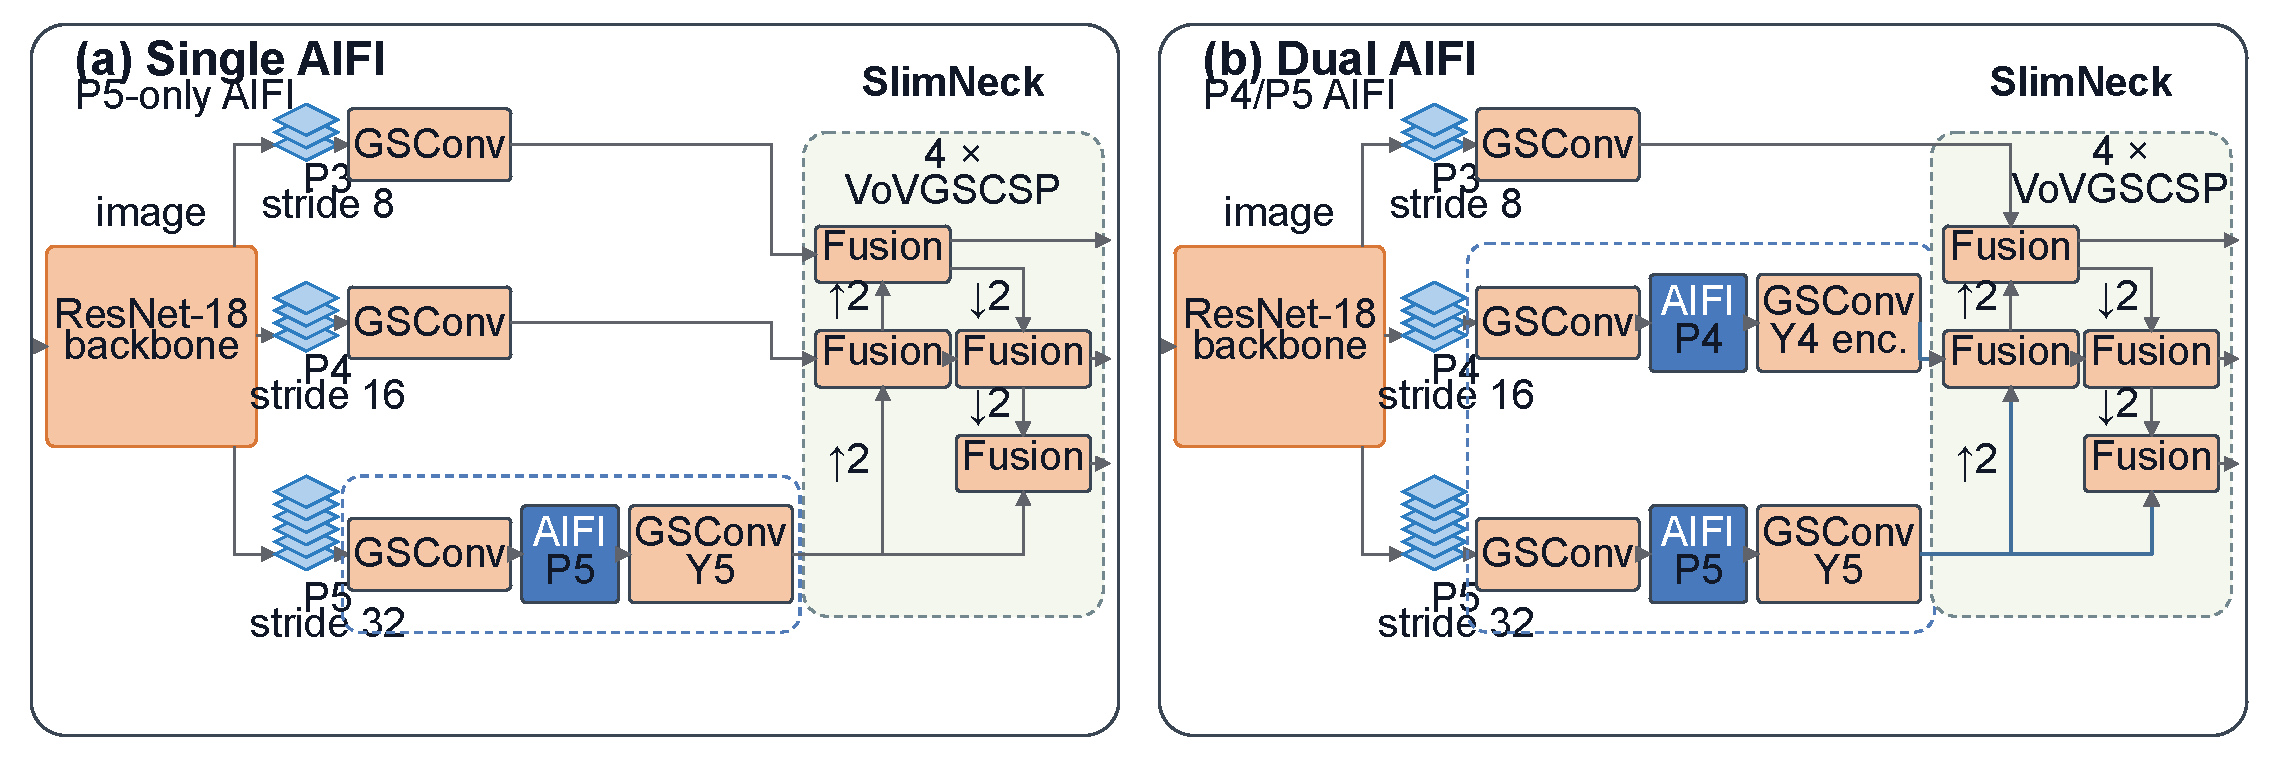
\includegraphics[width=\textwidth]{Fig1.pdf}
\caption{Comparison of single-scale and dual-scale intra-scale encoding. (a) A single AIFI branch encodes the projected P5 feature. (b) An additional, independently parameterized AIFI branch encodes the projected P4 feature before cross-scale fusion. Both panels share the same ResNet-18 backbone, GSConv projections, SlimNeck fusion, and decoder, so the P4 encoding branch---the additional AIFI layer together with its post-encoding projection---is the only structural difference between them. Each SlimNeck panel contains four VoVGSCSP fusion blocks, and $\uparrow_2$/$\downarrow_2$ denote nearest-neighbor upsampling and stride-two GSConv, respectively}
\label{fig:dual-aifi}
\end{figure*}

The combined model projects the backbone outputs to $d=256$ channels using GSConv-based operators $\Pi_l$. Independent AIFI layers $\mathcal{A}_4$ and $\mathcal{A}_5$ process the projected P4 and P5 features. Additional GSConv operators $\Gamma_4$ and $\Gamma_5$ prepare their outputs for fusion. Fig.~\ref{fig:overall} summarizes the complete inference and training arrangement.
\begin{figure*}[t]
\centering
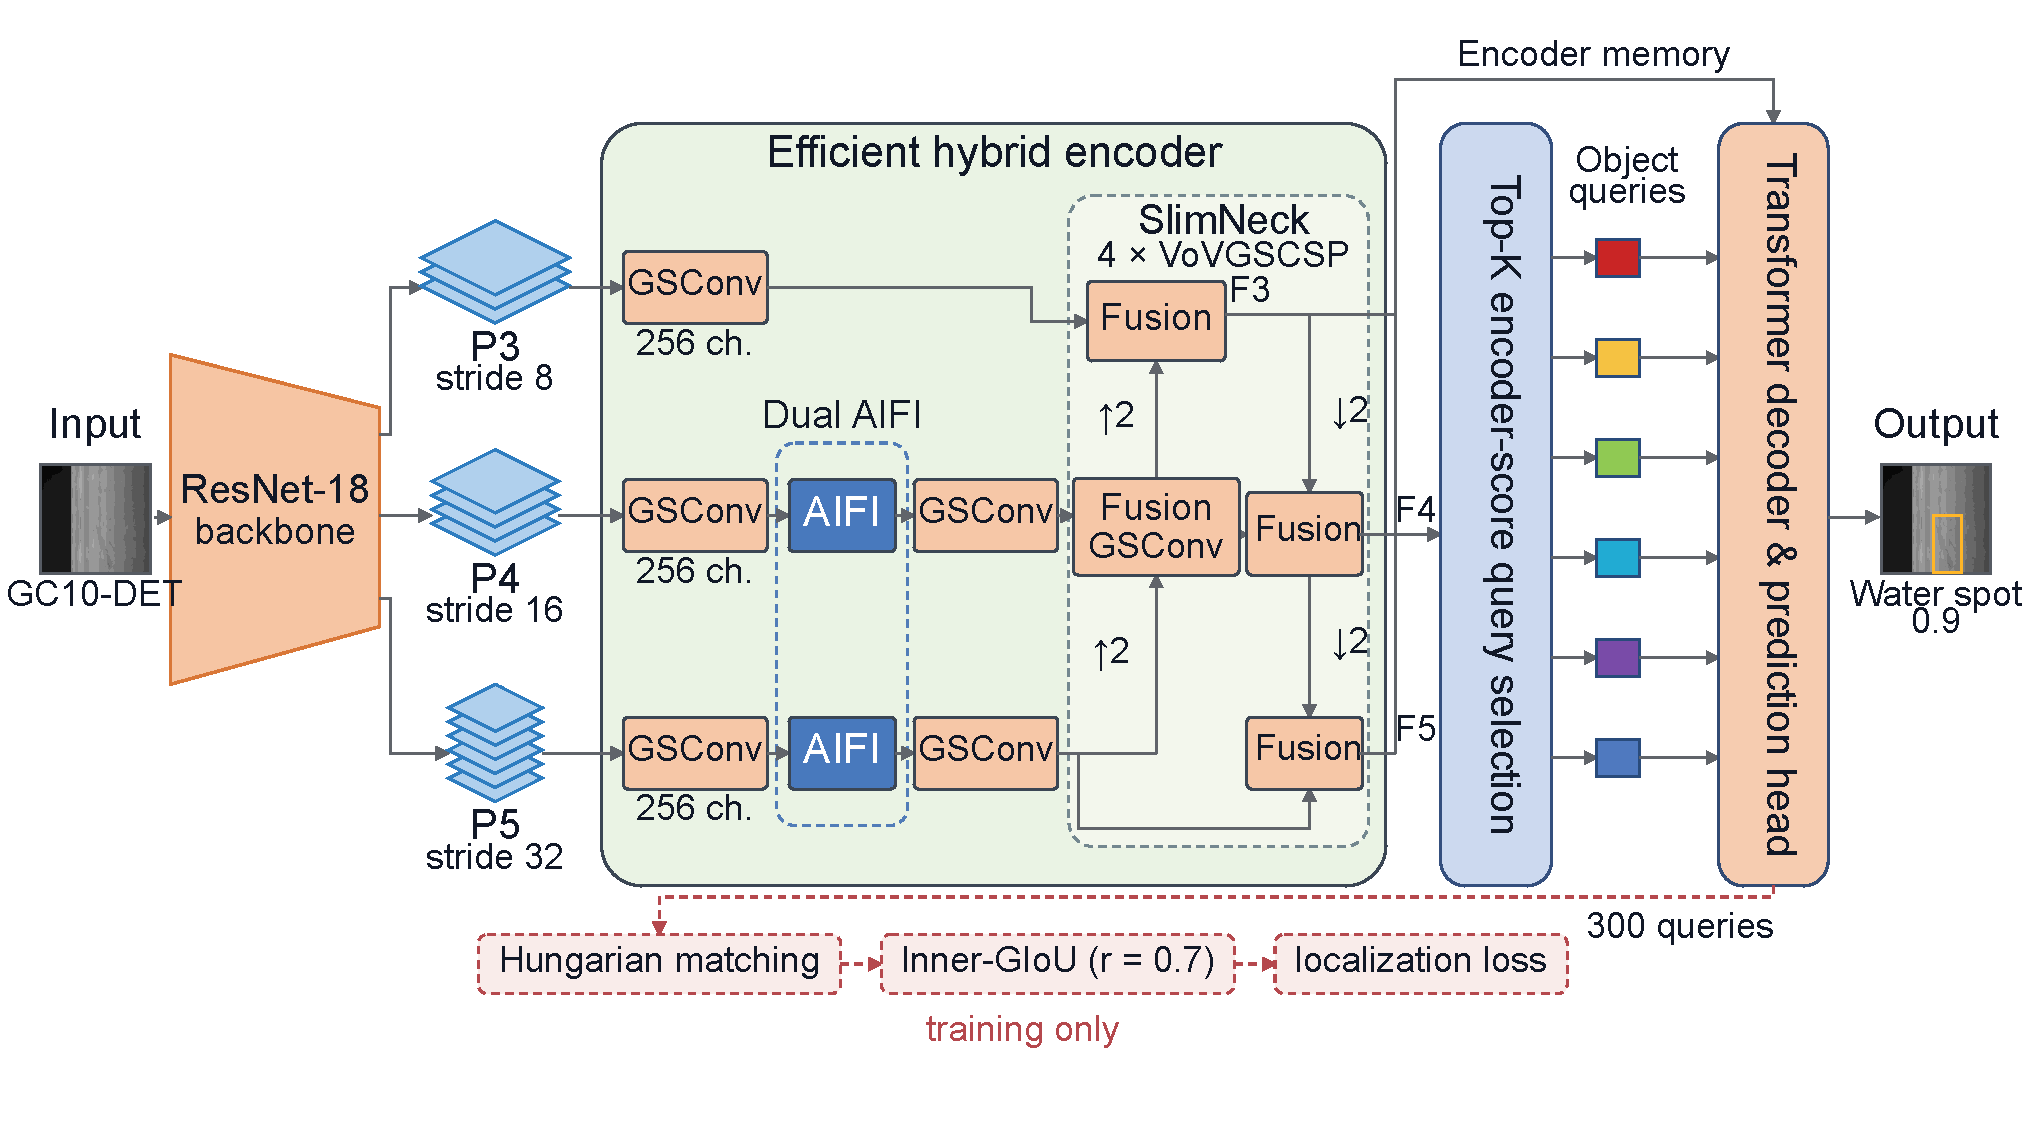
\includegraphics[width=\textwidth]{Fig2.pdf}
\caption{Overall architecture of the proposed RT-DETR-R18 adaptation. The inference path contains the ResNet-18 backbone, independent P4/P5 AIFI branches, GSConv-based SlimNeck fusion, and the unchanged decoder. The neck produces the three feature levels $F_3$, $F_4$, and $F_5$, each of which is projected per level before entering the decoder. The dashed branch below the decoder is active only during training: Hungarian matching uses the plain GIoU cost, and Inner-GIoU replaces only the overlap term of the regression loss, so neither contributes inference-time parameters. The input and output thumbnails are schematic vector renderings drawn for orientation}\label{fig:overall}
\end{figure*}
The resulting feature transformations are defined as:
\begin{equation}
\begin{aligned}
 X_3 &= \Pi_3(P_3),\\
 E_4 &= \Gamma_4\!\left(\mathcal{A}_4(\Pi_4(P_4))\right),\\
 E_5 &= \Gamma_5\!\left(\mathcal{A}_5(\Pi_5(P_5))\right).
\end{aligned}
\label{eq:encoder_branches}
\end{equation}
The two AIFI layers have separate parameters. Their outputs are fused with $X_3$ by the SlimNeck into three feature maps $F_3$, $F_4$, and $F_5$, from which the unchanged decoder $\mathcal{D}$ produces the final class scores and boxes $\widehat{\mathcal{Z}}$. Inner-GIoU enters only the training criterion and is absent from this inference graph.

For a projected feature $X_l\in\mathbb{R}^{B\times d\times H_l\times W_l}$, AIFI flattens the spatial dimensions into $T_l\in\mathbb{R}^{B\times N_l\times d}$, where $N_l=H_lW_l$. A two-dimensional sine--cosine positional embedding $S_l$ is added to the queries and keys, but not to the values. The implemented post-normalization encoder is
\begin{equation}
\begin{aligned}
 Q_l&=K_l=T_l+S_l,\qquad V_l=T_l,\\
 U_l&=\operatorname{LN}_1\!\left(T_l+\operatorname{MHA}(Q_l,K_l,V_l)\right),\\
 Z_l&=\operatorname{LN}_2\!\left(U_l+\operatorname{FFN}(U_l)\right).
\end{aligned}
\label{eq:aifi}
\end{equation}
Here, MHA, FFN, and LN denote multi-head attention, the feed-forward network, and layer normalization, respectively. The output $Z_l$ is reshaped to its original spatial layout. Each layer uses eight attention heads and a feed-forward network with hidden dimension 1024 and GELU activation; dropout is zero in the evaluated configuration. Channel projection occurs before AIFI rather than inside its attention operation.

P4 retains a finer spatial grid than P5, so its encoder can model relationships among intermediate-resolution features before cross-scale fusion; this is a design motivation, not direct evidence of enhanced texture discrimination. At an input size of $800\times800$, P4 and P5 contain 2500 and 625 tokens, so the P4 attention matrix has 16 times as many token pairs as the P5 matrix, which motivates the explicit cost evaluation in Section~\ref{sec:complexity}. The dual-scale variant also contains the post-encoding P4 projection $\Gamma_4$, so its measured effect cannot be attributed to attention alone.

\subsection{GSConv-based feature fusion}\label{sec:slimneck}

SlimNeck changes the feature-aggregation operators while preserving the three output resolutions. Following the GSConv design~\cite{li2024slimneck}, a primary convolution generates half of the output channels, and a depthwise convolution derives a complementary branch from those features. Fig.~\ref{fig:slimneck-modules} details the configured GSConv and VoVGSCSP forward paths. For an even output width $d_o$, the implemented operation is
\begin{equation}
\begin{aligned}
 A&=\mathcal{C}_{k,s}^{d_o/2}(X),\\
 B&=\mathcal{C}_{5,1}^{\mathrm{dw}}(A),\\
 \operatorname{GSConv}(X)&=\operatorname{Shuffle}([A,B]).
\end{aligned}
\label{eq:gsconv}
\end{equation}
The brackets denote channel concatenation. Each operator $\mathcal{C}$ comprises convolution, batch normalization, and the activation used in the implementation. The depthwise branch uses a $5\times5$ kernel. The primary features $A$ are computed once and reused; the branches do not apply two independent primary convolutions to $X$.

The fusion blocks use the implemented VoVGSCSP operator. Two $1\times1$ branches process the input; one passes through a sequence of GS bottlenecks, while the other forms a parallel path. Their outputs are concatenated and projected to the desired channel width:
\begin{equation}
 \mathcal{V}(X)=\mathcal{C}_{1,1}\!\left([
 \mathcal{C}_{1,1}^{a}(X),\,
 \mathcal{G}(\mathcal{C}_{1,1}^{b}(X))]\right),
\label{eq:vovgscsp}
\end{equation}
where $\mathcal{G}$ denotes the GS-bottleneck sequence. The final configuration uses three bottlenecks per fusion block and 256 output channels.

\begin{figure*}[t]
\centering
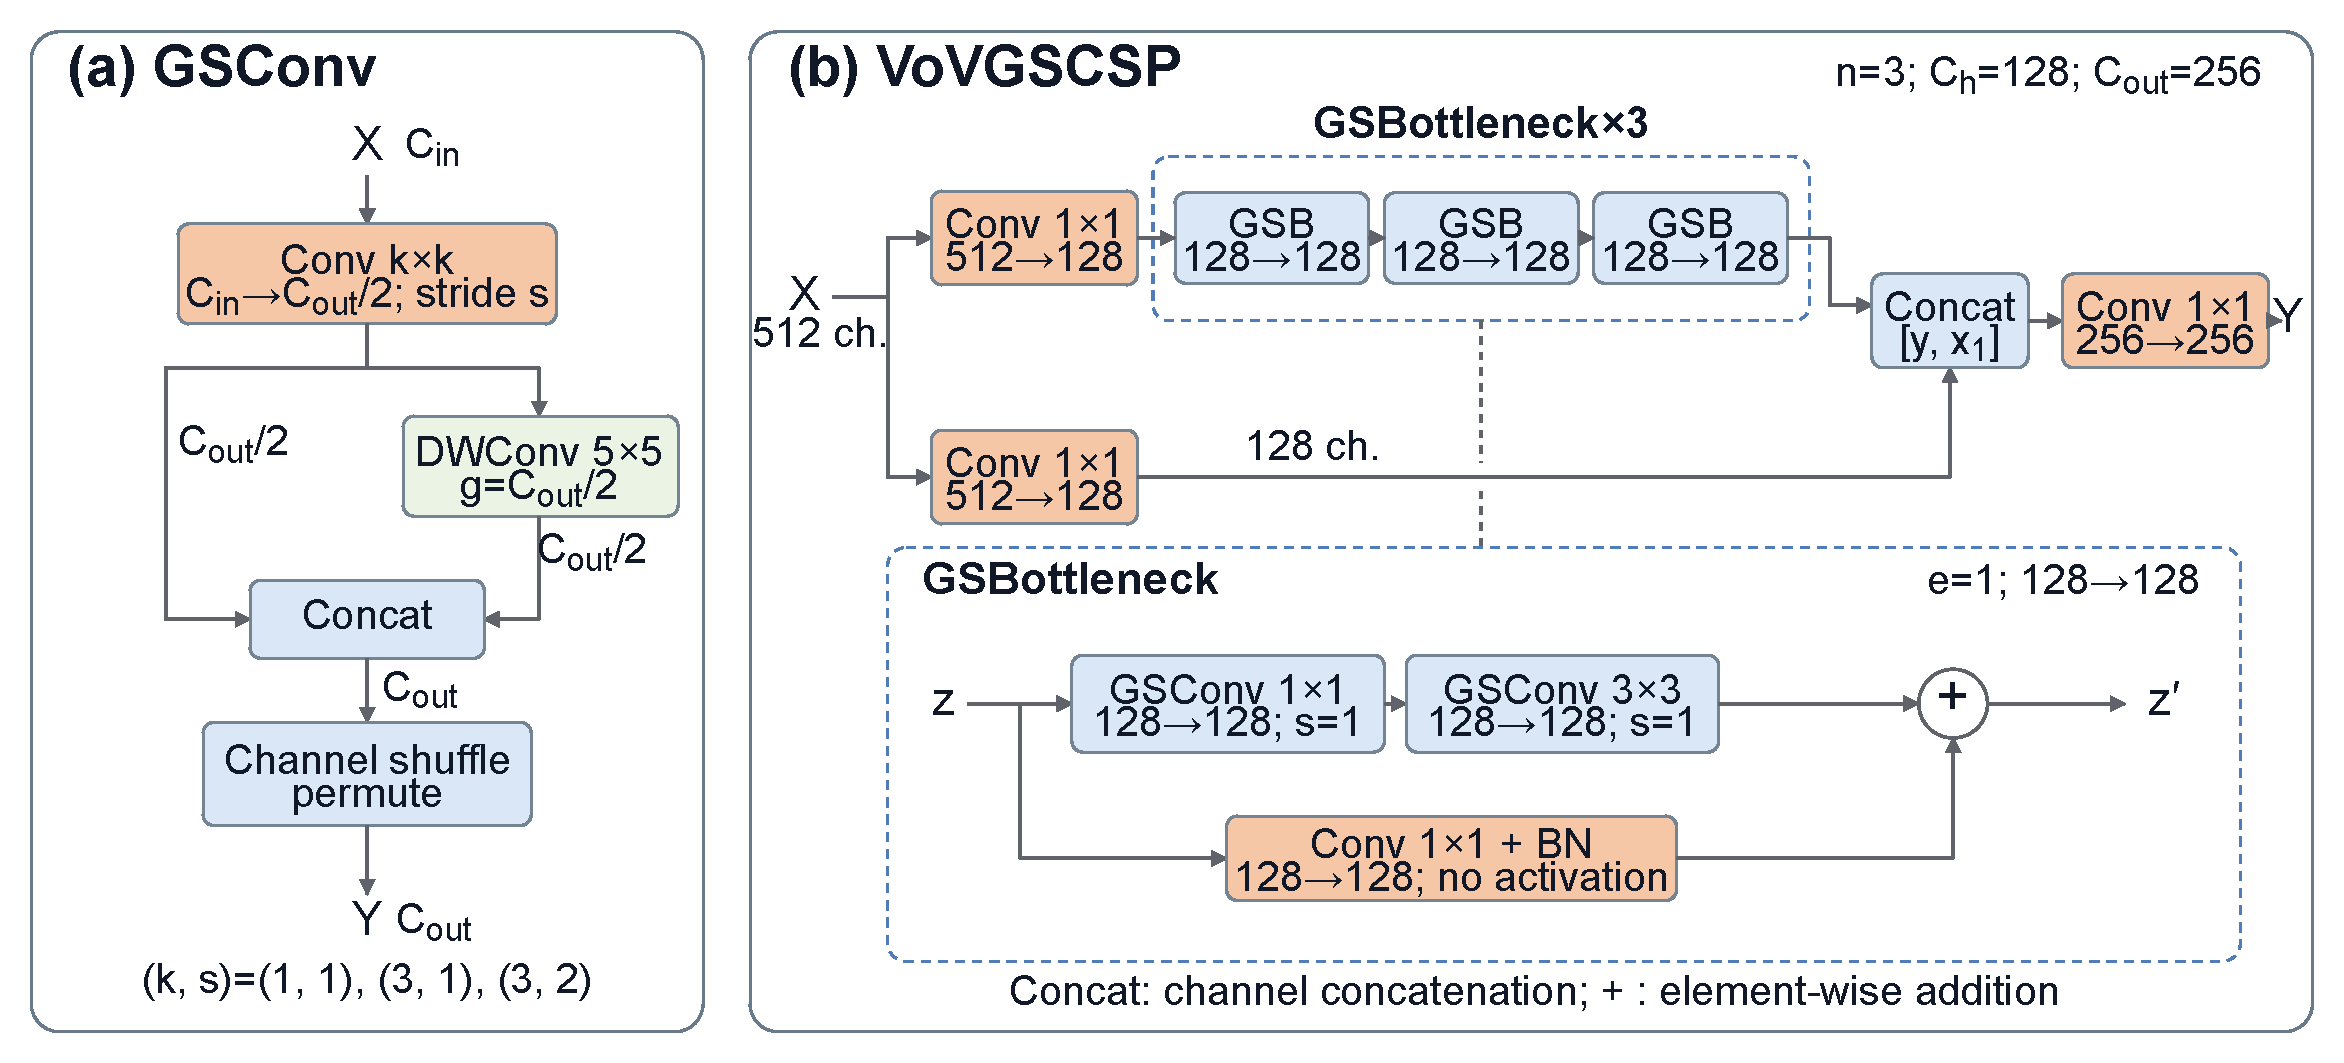
\includegraphics[width=\textwidth]{Fig3.pdf}
\caption{Forward-path details of the configured SlimNeck modules. (a) GSConv applies a standard $k\times k$ convolution, derives a depthwise $5\times5$ branch from its output, concatenates the two halves, and performs channel shuffling; the operator is instantiated with $(k,s)=(1,1)$, $(3,1)$, or $(3,2)$. (b) VoVGSCSP applies parallel $1\times1$ projections to the full 512-channel input, processes one 128-channel branch with three GS bottlenecks, concatenates the bypass and processed features, and projects the 256-channel result. Each GS bottleneck sums two GSConv layers with a $1\times1$ convolution plus batch-normalization shortcut. The schematic shows the executed forward path; the registered $3\times3$ residual convolution of the legacy VoVGSCSP implementation, which is not executed, is omitted}
\label{fig:slimneck-modules}
\end{figure*}

Let $\uparrow_2$ denote nearest-neighbor upsampling by two and $\downarrow_2$ denote stride-two GSConv. The top-down and bottom-up paths are expressed as
\begin{equation}
\begin{aligned}
 Y_4&=\Gamma_{\mathrm{td}}\!\left(\mathcal{V}_4^{\mathrm{td}}([\uparrow_2 E_5,E_4])\right),\\
 F_3&=\mathcal{V}_3^{\mathrm{td}}([\uparrow_2 Y_4,X_3]),\\
 F_4&=\mathcal{V}_4^{\mathrm{bu}}([\downarrow_2 F_3,Y_4]),\\
 F_5&=\mathcal{V}_5^{\mathrm{bu}}([\downarrow_2 F_4,E_5]).
\end{aligned}
\label{eq:neck}
\end{equation}
The output strides remain 8, 16, and 32, so the modification changes feature transformation and aggregation without introducing a fourth detection scale. It targets convolutional fusion cost, but its effect on end-to-end execution time must be measured rather than inferred from operator counts.

\subsection{Localization supervision and training objective}\label{sec:loss}

For a predicted box $B_p=(x_p,y_p,w_p,h_p)$ and a matched target $B_g$, auxiliary boxes retain their centers and scale their dimensions by $r$:
\begin{equation}
 B^{\mathrm{in}}(r)=(x,y,rw,rh),\qquad r=0.7.
\label{eq:inner_box}
\end{equation}
This setting shrinks the boxes. The resulting overlap is
\begin{equation}
 I_{\mathrm{in}}=
 \frac{|B_p^{\mathrm{in}}\cap B_g^{\mathrm{in}}|}
 {|B_p^{\mathrm{in}}\cup B_g^{\mathrm{in}}|+\epsilon}.
\label{eq:inner_iou}
\end{equation}
The implementation combines this auxiliary overlap with the GIoU enclosure penalty computed from the original boxes:
\begin{equation}
\begin{aligned}
 G_{\mathrm{in}}&= I_{\mathrm{in}}-\frac{A_c-A_u}{A_c},\\
 \mathcal{L}_{\mathrm{InnerGIoU}}&=1-G_{\mathrm{in}}.
\end{aligned}
\label{eq:inner_giou}
\end{equation}
Here, $A_c$ is the area of the smallest axis-aligned rectangle enclosing $B_p$ and $B_g$, and $A_u=|B_p\cup B_g|$. For readability, Eq.~\eqref{eq:inner_giou} does not repeat the numerical-stabilization term introduced in Eq.~\eqref{eq:inner_iou}. Equivalently, the loss replaces the ordinary IoU term in GIoU with an auxiliary-box IoU. It does not add a second, independent GIoU loss, nor does it apply a foreground mask to the input image.

Shrinking the auxiliary boxes changes the sensitivity of overlap to box displacement and scale. It does not, however, necessarily strengthen supervision for every poorly aligned pair: auxiliary boxes can become disjoint even when the original boxes overlap. In that case the original-box enclosure term is retained. The fixed ratio is a configuration choice in the present experiments, not a demonstrated optimum across datasets.

For each supervised prediction set, the criterion combines classification, L1 regression, and the selected geometric term:
\begin{equation}
 \mathcal{L}_{\mathrm{det}}
 =\mathcal{L}_{\mathrm{cls}}+5\mathcal{L}_{1}+2\mathcal{L}_{\mathrm{geo}}.
\label{eq:loss}
\end{equation}
The baseline uses $\mathcal{L}_{\mathrm{geo}}=1-\operatorname{GIoU}$, whereas the configurations with Inner-GIoU use $\mathcal{L}_{\mathrm{InnerGIoU}}$. The implementation enables Varifocal classification supervision, with a focal-loss fallback when no targets are present~\cite{zhang2021varifocalnet}. Encoder predictions, auxiliary decoder outputs, and denoising outputs receive the corresponding detection losses, and their contributions are summed with the final decoder loss during training.

Hungarian assignment remains based on classification, L1 distance, and ordinary GIoU, with cost weights 2, 5, and 2. The Inner-GIoU substitution therefore modifies regression supervision, not the matching cost or the IoU quality targets used for classification. At inference, the detector executes only the backbone, encoder, fusion neck, and decoder. The evaluated RT-DETR prediction path does not apply external non-maximum suppression, and the training-only loss introduces no additional inference operation.

\section{Experiments and results}\label{sec:experiments}

\subsection{Datasets and experimental protocol}\label{sec:protocol}

GC10-DET is the primary benchmark, covering ten metallic surface defect categories~\cite{lv2020gc10}. The experiments use the project-specific 2292-image collection, partitioned into 1833 training, 229 validation, and 230 test images. These counts describe the collection used here, not the full 3570-image release reported in the original dataset paper. The group-aware partition was generated once on a cloud server and frozen for all GC10-DET comparisons: images sharing the filename-prefix group identifier were assigned to the same partition, and training seeds changed initialization and stochastic training operations but not dataset membership. The split targets class balance at image and object-instance levels while retaining the prescribed partition sizes.

NEU-DET is the secondary benchmark. It contains 1800 images in six categories whose distribution differs from GC10-DET, which provides a separate test of the design's applicability~\cite{he2020neudet}. The baseline and combined model were trained on NEU-DET and evaluated on its held-out test partition; a GC10-DET-trained model was not evaluated directly on NEU-DET. Dataset-specific input sizes were $800\times800$ for GC10-DET and $640\times640$ for NEU-DET.

The principal R18 experiments used random seeds 0, 1, and 2, a batch size of 8, and a maximum of 300 epochs. Early stopping used a patience of 50 epochs, and the best validation checkpoint was evaluated on the test partition. Recorded configurations specify AdamW, an initial learning rate of $10^{-4}$, a weight-decay setting of $10^{-4}$, automatic mixed precision, and eight data-loader workers. The learning-rate multiplier after warm-up is constant in the recorded configuration. Although the configuration field is named \texttt{warmup\_epochs}, the project trainer interprets its value of 2000 as a number of training iterations---an implementation detail that matters for reproducing the schedule. Recorded augmentation settings include horizontal flipping with probability 0.5, translation magnitude 0.1, scale variation 0.5, and no mosaic or mixup. These settings are shared by the R18 comparisons; the reference detectors are not assumed to share their optimization behavior.

Accuracy is evaluated using the mean average precision (mAP) metrics mAP50, mAP75, and mAP50--95, which average class-wise average precision (AP) at IoU thresholds of 0.50, at 0.75, and over ten thresholds from 0.50 to 0.95 in steps of 0.05, respectively. mAP50--95 is the principal summary metric; the other thresholds reveal differences in overlap sensitivity. The principal metric reflects both recognition and localization and is not an isolated measure of regression quality.

Precision, recall, and F1 are macro-averaged over categories. Class-wise F1 is calculated before averaging, so the reported F1 is not the harmonic mean of the reported mean precision and recall. The evaluator selects the operating point from the maximum of a smoothed mean F1 curve at IoU 0.50; these values are descriptive summaries of the test curve, not performance at a deployment threshold fixed on validation data. Unless stated otherwise, results are percentages expressed as the mean and sample standard deviation across the three seeds, and differences are reported in percentage points. No statistical-significance claim is made from three runs alone.

\subsection{Primary results on GC10-DET}\label{sec:gc10}

Table~\ref{tab:gc10ablation} compares the baseline, three single-component variants, three pairwise combinations, and the combined model. All eight configurations use the same R18 backbone and decoder interface, forming a complete $2^3$ factorial design. A background here denotes a fixed subset of components, including the empty set, against which the marginal effect of adding the dual-scale branch can be isolated.

\begin{table*}[t]
\centering
\caption{Ablation results on the frozen GC10-DET test partition. All entries are percentages, reported as mean $\pm$ sample standard deviation over seeds 0--2. The component columns mark the complete $2^3$ factorial design: SlimNeck (SN), Inner-GIoU (IG), dual-scale AIFI (DA); ``Combined'' is all three.}
\label{tab:gc10ablation}
\scriptsize
\setlength{\tabcolsep}{3.5pt}
\begin{adjustbox}{max width=\textwidth}
\begin{tabular}{@{}lccccccccc@{}}
\toprule
Configuration & SN & IG & DA & Precision & Recall & F1 & mAP50 & mAP75 & mAP50--95 \\
\midrule
RT-DETR-R18 & -- & -- & -- & 56.64 $\pm$ 7.82 & 55.69 $\pm$ 1.59 & 53.23 $\pm$ 2.90 & 54.42 $\pm$ 2.19 & 25.79 $\pm$ 4.53 & 28.01 $\pm$ 1.04 \\
SN & $\checkmark$ & -- & -- & 71.32 $\pm$ 3.79 & 57.74 $\pm$ 1.18 & 60.67 $\pm$ 1.14 & 59.58 $\pm$ 3.04 & 26.15 $\pm$ 0.39 & 29.78 $\pm$ 0.70 \\
IG & -- & $\checkmark$ & -- & 67.54 $\pm$ 1.74 & 57.54 $\pm$ 4.24 & 59.21 $\pm$ 2.62 & 58.73 $\pm$ 1.64 & 24.55 $\pm$ 1.02 & 29.17 $\pm$ 0.56 \\
DA & -- & -- & $\checkmark$ & 70.65 $\pm$ 0.70 & 55.43 $\pm$ 2.50 & 58.45 $\pm$ 2.09 & 57.62 $\pm$ 0.70 & 24.12 $\pm$ 0.70 & 29.10 $\pm$ 0.66 \\
SN + IG & $\checkmark$ & $\checkmark$ & -- & 70.95 $\pm$ 5.99 & 56.31 $\pm$ 2.46 & 59.69 $\pm$ 3.50 & 58.17 $\pm$ 2.05 & 27.48 $\pm$ 0.16 & 30.23 $\pm$ 1.04 \\
SN + DA & $\checkmark$ & -- & $\checkmark$ & 71.06 $\pm$ 4.56 & 55.64 $\pm$ 1.44 & 59.02 $\pm$ 1.56 & 57.56 $\pm$ 1.29 & 26.04 $\pm$ 0.27 & 29.43 $\pm$ 0.66 \\
IG + DA & -- & $\checkmark$ & $\checkmark$ & 69.94 $\pm$ 1.57 & 56.42 $\pm$ 0.25 & 58.90 $\pm$ 0.76 & 56.99 $\pm$ 0.46 & 26.33 $\pm$ 3.68 & 29.37 $\pm$ 1.39 \\
Combined & $\checkmark$ & $\checkmark$ & $\checkmark$ & 71.34 $\pm$ 3.43 & 60.92 $\pm$ 1.02 & 62.81 $\pm$ 0.34 & 61.00 $\pm$ 1.16 & 25.65 $\pm$ 2.79 & 30.29 $\pm$ 0.90 \\
\botrule
\end{tabular}
\end{adjustbox}
\end{table*}

Each single-component variant increased mean mAP50--95 relative to the baseline, with SlimNeck producing the largest increase. Inner-GIoU and dual-scale AIFI, however, had lower mAP75 than the baseline, so neither gain can be read as uniformly better localization across overlap thresholds.

The combined model achieved 61.00\% mAP50 and 30.29\% mAP50--95, exceeding the baseline by 6.58 and 2.28 percentage points, with mean recall and F1 up by 5.23 and 9.58 percentage points; mAP75, by contrast, decreased from 25.79\% to 25.65\%. The evidence is therefore strongest for overall detection performance, most clearly at IoU 0.50, not for high-overlap box alignment.

The complete factorial design qualifies this incremental picture. Across the four backgrounds, the mean paired per-seed change in mAP50--95 when adding the dual-scale branch ranges from $-0.35$ to $+1.09$ percentage points, and the sign of the per-seed change is inconsistent within every background; each mean change is smaller than the standard deviation of its own three paired differences (0.42--1.65 points), so these shifts are no larger than run-to-run variation. Both pairwise combinations containing the branch fall short of SlimNeck with Inner-GIoU on mAP50--95, and their mAP75 values sit between those of the baseline and SlimNeck--Inner-GIoU, so adding the branch to a single-component background produces no consistent high-overlap penalty. On the strongest two-component background the branch does change the detection trade-off: it increases mAP50 by 2.84 points and recall by 4.61 points, with positive per-seed differences in all three runs, yet mAP50--95 increases by only 0.06 points while mAP75 decreases by 1.83 points. On that background, the branch therefore yields a seed-consistent gain at loose overlap thresholds, but not under the principal metric.

Paired per-seed results show higher mAP50--95 for the combined model in all three runs (31.21, 29.41, and 30.25\% against 27.17, 27.69, and 29.18\% for the baseline), with the same pattern for mAP50, recall, and F1, whereas mAP75 decreases for seed 2. This consistency supports the observed advantage under the fixed partition, without implying significance across other partitions or acquisition conditions.

\begin{table*}[t]
\centering
\caption{Reference-detector comparison on the same GC10-DET test partition at an input size of $800\times800$. Values are percentages, reported as mean $\pm$ sample standard deviation over seeds 0--2.}
\label{tab:gc10reference}
\scriptsize
\setlength{\tabcolsep}{4pt}
\begin{adjustbox}{max width=\textwidth}
\begin{tabular}{@{}lcccccc@{}}
\toprule
Model & Precision & Recall & F1 & mAP50 & mAP75 & mAP50--95 \\
\midrule
RT-DETR-R18 & 56.64 $\pm$ 7.82 & 55.69 $\pm$ 1.59 & 53.23 $\pm$ 2.90 & 54.42 $\pm$ 2.19 & 25.79 $\pm$ 4.53 & 28.01 $\pm$ 1.04 \\
RT-DETR-R50 & 67.77 $\pm$ 2.50 & 56.94 $\pm$ 1.79 & 59.39 $\pm$ 2.11 & 56.06 $\pm$ 2.04 & 27.78 $\pm$ 2.25 & 29.63 $\pm$ 0.53 \\
YOLOv8n & 62.39 $\pm$ 8.63 & 49.17 $\pm$ 3.23 & 50.60 $\pm$ 1.73 & 50.49 $\pm$ 1.17 & 22.87 $\pm$ 1.89 & 24.57 $\pm$ 0.86 \\
YOLOv8s & 59.96 $\pm$ 3.27 & 50.93 $\pm$ 3.19 & 51.95 $\pm$ 2.28 & 52.46 $\pm$ 1.46 & 24.03 $\pm$ 0.82 & 25.86 $\pm$ 0.43 \\
Combined RT-DETR-R18 & 71.34 $\pm$ 3.43 & 60.92 $\pm$ 1.02 & 62.81 $\pm$ 0.34 & 61.00 $\pm$ 1.16 & 25.65 $\pm$ 2.79 & 30.29 $\pm$ 0.90 \\
\botrule
\end{tabular}
\end{adjustbox}
\end{table*}

Table~\ref{tab:gc10reference} places these results alongside RT-DETR-R50 and YOLOv8n/s. The combined model obtained the highest mean mAP50 and mAP50--95 among these tested detectors, exceeding RT-DETR-R50 by 4.94 and 0.66 percentage points, respectively; the mAP50--95 margin is smaller than the combined model's own seed-to-seed standard deviation (0.90 points), and RT-DETR-R50 achieved higher mAP75. These are comparisons under the present training and evaluation protocols, not evidence of universal superiority; in particular, differences in capacity, preprocessing, and optimization prevent the YOLO comparisons from being read as controlled single-factor ablations.

\begin{table}[!tbp]
\centering
\caption{Category-wise GC10-DET AP50--95, averaged over three seeds. Changes are computed before rounding and expressed in percentage points.}
\label{tab:classes}
\scriptsize
\begin{tabular*}{\columnwidth}{@{\extracolsep{\fill}}lccc@{}}
\toprule
Category & Baseline & Combined & Change \\
\midrule
Punching & 57.48 & 57.74 & +0.25 \\
Weld line & 45.02 & 46.95 & +1.93 \\
Crescent gap & 53.67 & 55.81 & +2.14 \\
Water spot & 35.32 & 36.63 & +1.31 \\
Oil spot & 18.50 & 24.30 & +5.80 \\
Silk spot & 13.61 & 15.27 & +1.66 \\
Inclusion & 6.56 & 7.86 & +1.31 \\
Rolled pit & 19.25 & 21.94 & +2.70 \\
Crease & 19.58 & 22.07 & +2.48 \\
Waist folding & 11.15 & 14.32 & +3.17 \\
\botrule
\end{tabular*}
\end{table}

Category-level results in Table~\ref{tab:classes} show higher mean AP50--95 for all ten categories, with increases ranging from 0.25 points for punching to 5.80 points for oil spot; inclusion remained difficult at 7.86\% AP50--95 despite improvement. The aggregate gain is therefore not confined to one category, but weak or irregular defects remain unsolved; category labels alone do not establish whether gains arise from small-object recognition, texture modeling, or more accurate regression.

\subsection{Secondary results on NEU-DET}\label{sec:neu}

Table~\ref{tab:neu} reports the independently trained baseline and combined model on NEU-DET. The combined model reached 73.19\% mAP50 and 44.23\% mAP50--95, compared with 72.47\% and 43.57\% for the baseline. The gains are smaller than those on the primary dataset in precision, recall, F1, mAP50, and mAP50--95, whereas mAP75 improves by 1.05 points.

\begin{table*}[t]
\centering
\caption{Secondary-benchmark results on NEU-DET. Models are trained on NEU-DET, rather than transferred directly from GC10-DET. Entries are percentages, reported as mean $\pm$ sample standard deviation over seeds 0--2. The change row is computed before rounding, so it may differ from the difference of the rounded means.}
\label{tab:neu}
\scriptsize
\setlength{\tabcolsep}{4pt}
\begin{adjustbox}{max width=\textwidth}
\begin{tabular}{@{}lcccccc@{}}
\toprule
Model & Precision & Recall & F1 & mAP50 & mAP75 & mAP50--95 \\
\midrule
RT-DETR-R18 & 72.95 $\pm$ 2.17 & 67.50 $\pm$ 0.67 & 68.87 $\pm$ 1.63 & 72.47 $\pm$ 0.99 & 45.65 $\pm$ 1.10 & 43.57 $\pm$ 0.51 \\
Combined RT-DETR-R18 & 75.65 $\pm$ 3.26 & 67.55 $\pm$ 1.61 & 70.38 $\pm$ 0.78 & 73.19 $\pm$ 0.51 & 46.69 $\pm$ 0.30 & 44.23 $\pm$ 0.39 \\
\midrule
Change (percentage points) & +2.70 & +0.05 & +1.50 & +0.72 & +1.05 & +0.65 \\
\botrule
\end{tabular}
\end{adjustbox}
\end{table*}

Per-seed paired differences in mAP50--95 were positive in all three runs (+1.59, +0.09, and +0.27 percentage points), and category-level behavior was nonuniform: mean AP50--95 increased by 3.22 points for rolled-in scale and 1.34 for pitted surface but decreased by 0.80 for crazing and 0.76 for patches. The second benchmark therefore supports a modest aggregate benefit after dataset-specific training, not a universal gain across defect categories; without a full NEU-DET ablation, the individual contributions of the three components cannot be separated on this dataset.

\subsection{Computational cost and practical limitations}\label{sec:complexity}

Table~\ref{tab:complexity} separates structural measurements from recorded execution time. Parameters are counted from model tensors, and operation counts come from the project's THOP-based profiling procedure, with a multiply--add counted as two operations; the reported counts should be read within that profiler's operator coverage, which has not been independently validated for every attention operation.

\begin{table*}[t]
\centering
\caption{Model complexity and batch-one forward latency at $800\times800$ in FP32, measured in a single session on an idle NVIDIA RTX 4090 (driver 595.71.05; PyTorch 2.5.1, CUDA 12.4) with 100 warm-up and 500 timed iterations per model. Operation counts follow the project THOP procedure; peak memory is the maximum CUDA allocation during the timed passes; latency statistics describe iteration-level variation, not across-seed variation. SD, standard deviation; P50/P95, median and 95th-percentile latency; FPS, frames per second. SN and DA follow Table~\ref{tab:gc10ablation}. IG is omitted: its inference graph is identical to the baseline.}
\label{tab:complexity}
\scriptsize
\setlength{\tabcolsep}{3.5pt}
\begin{tabular*}{\textwidth}{@{\extracolsep{\fill}}lccccccc@{}}
\toprule
Model & Params (M) & GFLOPs & Mean $\pm$ SD (ms) & P50 (ms) & P95 (ms) & FPS & Peak mem.\ (MiB) \\
\midrule
RT-DETR-R18 & 19.88 & 88.04 & 15.35 $\pm$ 0.76 & 15.24 & 15.35 & 65.16 & 281 \\
SN & 19.31 & 82.26 & 18.69 $\pm$ 1.07 & 18.53 & 18.69 & 53.50 & 277 \\
DA & 20.74 & 91.00 & 17.95 $\pm$ 1.45 & 17.55 & 21.20 & 55.70 & 606 \\
SN + IG & 19.31 & 82.26 & 18.57 $\pm$ 0.94 & 18.43 & 18.64 & 53.86 & 277 \\
SN + DA & 20.14 & 85.07 & 22.64 $\pm$ 3.22 & 20.96 & 31.19 & 44.18 & 603 \\
IG + DA & 20.74 & 91.00 & 18.77 $\pm$ 2.75 & 17.65 & 26.45 & 53.27 & 606 \\
Combined & 20.14 & 85.07 & 21.74 $\pm$ 2.67 & 20.87 & 29.83 & 45.99 & 603 \\
RT-DETR-R50 & 41.97 & 200.54 & 26.31 $\pm$ 2.58 & 25.52 & 33.48 & 38.00 & 491 \\
\botrule
\end{tabular*}
\end{table*}

SlimNeck alone reduced registered parameters from 19.88 to 19.31 million and profiler-reported operations from 88.04 to 82.26 GFLOPs, while Inner-GIoU left the inference architecture unchanged. The dual-scale branch adds roughly 0.85 million parameters through its second AIFI layer and projections, and the combined model has 1.26\% more parameters but 3.37\% fewer reported operations than the baseline: the final design is not smaller by parameter count. The legacy VoVGSCSP implementation also registers a convolution that its forward path never calls; those unused parameters are not treated as active feature processing.

The timing script measures forward passes on a synthetic batch-one input with synchronized CUDA events, excluding image decoding, preprocessing, and post-processing; FPS is calculated as $1000$ divided by mean latency in milliseconds, and no production-line throughput claim is inferred.

Per-image latency standard deviations ranged from 0.76 to 3.22\,ms across the 500 timed iterations. The combined model averaged 21.74\,ms per image (45.99 FPS) against 15.35\,ms (65.16 FPS) for the baseline, a 42\% increase measured on this GPU. Memory is the more pronounced cost: every configuration containing the dual-scale branch required 603--606\,MiB of peak CUDA memory, slightly more than twice the 281\,MiB of the baseline, consistent with the 2500-token P4 attention maps. SlimNeck ran slower than the baseline despite fewer reported operations, so on this hardware its depthwise-and-shuffle operators execute less efficiently than the dense convolutions they replace: lower profiler-reported GFLOPs do not imply faster execution.

The SlimNeck--Inner-GIoU variant already reached 30.23\% mAP50--95 on GC10-DET, close to the combined model's 30.29\%, while running 3.2\,ms faster per image and using less than half of its peak memory. Dual-scale processing raised mAP50 and recall but produced no consistent mAP50--95 gain in any background, and it doubled the memory footprint. The two-component variant is therefore the preferable configuration when high-overlap accuracy, latency, or memory is prioritized. The present evidence does not justify selecting the combined model for every operating requirement.

Several limitations bound the conclusions. Three seeds characterize only limited training variability, not uncertainty over acquisition sites or dataset partitions. A shared frozen split improves comparability, but it does not remove annotation uncertainty, class imbalance, or selection bias. The Inner-GIoU scale ratio was fixed rather than swept, so no claim about an optimal ratio is possible. Latency and memory were measured on a single GPU in FP32, and absolute figures may shift on other hardware or precisions. The reference-detector set is limited and does not establish state-of-the-art performance against current detection systems. Independently training on NEU-DET demonstrates applicability to a second benchmark, not robustness to unseen industrial domains. These limitations motivate broader comparisons and hardware-diverse profiling rather than stronger claims based on the existing measurements.

\section{Conclusion}\label{sec:conclusion}

This study evaluated an RT-DETR-R18 adaptation combining GSConv-based SlimNeck, independent P4/P5 AIFI encoding, and Inner-GIoU regression supervision. On the primary GC10-DET benchmark, the combined model exceeded the baseline by 6.58 and 2.28 percentage points in mAP50 and mAP50--95 across three seeds, with higher mean AP50--95 in all ten defect categories (from +0.25 to +5.80 points); separate training and testing on NEU-DET produced a smaller increase from 43.57\% to 44.23\% mAP50--95. Across the complete factorial ablation, the dual-scale branch had no consistent marginal effect on mAP50--95 in any background, although it improved mAP50 and recall on the strongest two-component configuration in all three runs. Its measurable cost is a doubling of peak inference memory, while the full model still reached about 46 FPS on the test GPU; GC10-DET mAP75 did not improve over the baseline. The SlimNeck--Inner-GIoU variant is therefore the preferable configuration when memory or high-overlap accuracy is prioritized. The result is an accuracy-oriented adaptation with a characterized memory cost, not a smaller or faster detector. Future work should prioritize memory-efficient attention at intermediate resolutions, Inner-GIoU ratio sensitivity, and evaluation under additional industrial acquisition conditions.

\backmatter
\section*{Statements and Declarations}
\bmhead{Funding}
The authors declare that no funds, grants, or other support were received during the preparation of this manuscript.
\bmhead{Competing interests}
The authors have no relevant financial or non-financial interests to disclose.
\bmhead{Data availability}
The experiments use two publicly available benchmark datasets: GC10-DET, described by Lv et al.~\cite{lv2020gc10}, and NEU-DET, described by He et al.~\cite{he2020neudet}. Both datasets are obtainable through the sources specified in these original publications. The fixed train/test partition of GC10-DET used for all compared configurations, and the separate NEU-DET split used for the secondary benchmark, are recorded in the dataset preparation files of the repository described under Code availability.
\bmhead{Code availability}
The implementation, training configurations, evaluation scripts, and the dataset preparation files defining the splits used in all reported experiments are available at \url{https://github.com/web-wjm/RT-DETR}.
\bmhead{Author contributions}
Jiaming Wu: methodology, software, validation, formal analysis, and writing---original draft. Yong Chen: data curation, investigation, visualization, and writing---review and editing. Xianggong Hong: conceptualization, supervision, and writing---review and editing. All authors read and approved the final manuscript.
\bmhead{Ethics and consent declarations}
Not applicable. This study uses only publicly available industrial surface-defect image datasets and involves no human participants, personal data, or animals.

\bibliography{sn-bibliography}
\end{document}
